\documentclass[10 pt,usenames,dvipsnames, oneside]{article}
\usepackage{../../../modelo-ensino-medio}


\begin{document}

\begin{center}
  \begin{minipage}[l]{3cm}

\includegraphics[width=2cm]{logo}    
\end{minipage}\hfill
\begin{minipage}[r]{.8\textwidth}
 {\Large \scshape Atividade: Arremesso}  
\end{minipage}
\end{center}
\vspace{.2cm}

\ifdefined\prof
\begin{objetivos}
\item \textbf{LAF2} Compreender a taxa de variação como uma medida de covariação entre grandezas e utilizá-la para interpretar situações reais.
\end{objetivos}

\begin{goals}
\begin{enumerate}

\item [OE1] Construir, a partir de uma situação real de lançamento oblíquo, a ideia de taxa de variação instantânea.

\item [OE2] Usar a intuição sobre velocidade inicial instantânea e velocidade nula (ausência de movimento) para comparar com o limite das taxas de variação média.

\end{enumerate}

\tcblower

\begin{itemize}

\item Nessa atividade a ideia informal de limite é explorada através de cálculos de taxas de
variação em intervalos sucessivos de comprimento cada vez menor.
\item Caso seja possível utilizar recursos computacionais, é interessante fazer os cálculos em
uma planilha eletrônica com intervalos ainda menores para ilustrar a convergência.
\item Discuta a ideia da aproximação geometricamente: retas secantes que se aproximam da
reta tangente. A intenção aqui é apenas construir modelos para formar algum tipo de
intuição sobre o assunto, não pretendemos tratar as coisas de maneira formal.

\begin{figure}[H]
\centering

  \begin{tikzpicture}[xscale=2.8,scale=1.1]
  \clip (-.5,-.5) rectangle (1.6,4.4);
    \draw [->, thick] (0,0) -- (0,4.4);
    \node[left, rotate=90] at (-.25,4) {altura (h)};
    \draw [->, thick] (0,0) -- (1.6,0) node [below left, yshift=-.45cm] {tempo (t)};
    \foreach \x in {0.5,1,1.5,2} \draw (\x,.1)  -- (\x,-.1)  node[below] {\x};
    \foreach \y in {1,...,4} \draw (.03571,\y) -- (-.03571,\y) node[left] {\y};        
    \node[below left] at (0,0) {0};
    \draw [domain=0:1.5, color=session3, smooth, very thick] plot (\x,-5*\x^2 +6*\x + 2.1);
    \draw [domain=-1:1.5, very thick, session2, dashed] plot (\x,{6*\x+2.1});
    \draw [domain=-1:1.5, thick] plot (\x,{4*\x+2.1});
    \draw [domain=-1:1.5, thick] plot (\x,{3*\x+2.1});
    \draw [domain=-1:1.5, thick] plot (\x,{2*\x+2.1});
    \draw [domain=-1:1.5, thick] plot (\x,{\x+2.1});



  \end{tikzpicture}
\end{figure}



\item Após o término da atividade discuta com os estudantes um pouco mais sobre o conceito
de taxa de variação (velocidade) instantânea. Utilize outros exemplos: o velocímetro do
carro (o que significa quando o ponteiro marca 50km/h?); o custo marginal de
produção de um determinado produto, dentre outros.

\item Essa atividade está disponível em uma versão digital no link: \url{https://teacher.desmos.com/activitybuilder/custom/5de193196148282ac346889a}

\end{itemize}

\end{goals}

\bigskip
\begin{center}
{\large \scshape Atividade}
\end{center}
\fi

Um jogador de basquete ao lançar a bola em direção à cesta a vê descrever uma curva no ar chamada \textit{parábola}. Essa curva é resultado da combinação de dois movimentos: um na direção horizontal, responsável por fazer a bola "ir para frente" e outro na direção vertical que faz a bola "subir e descer".

\begin{center}
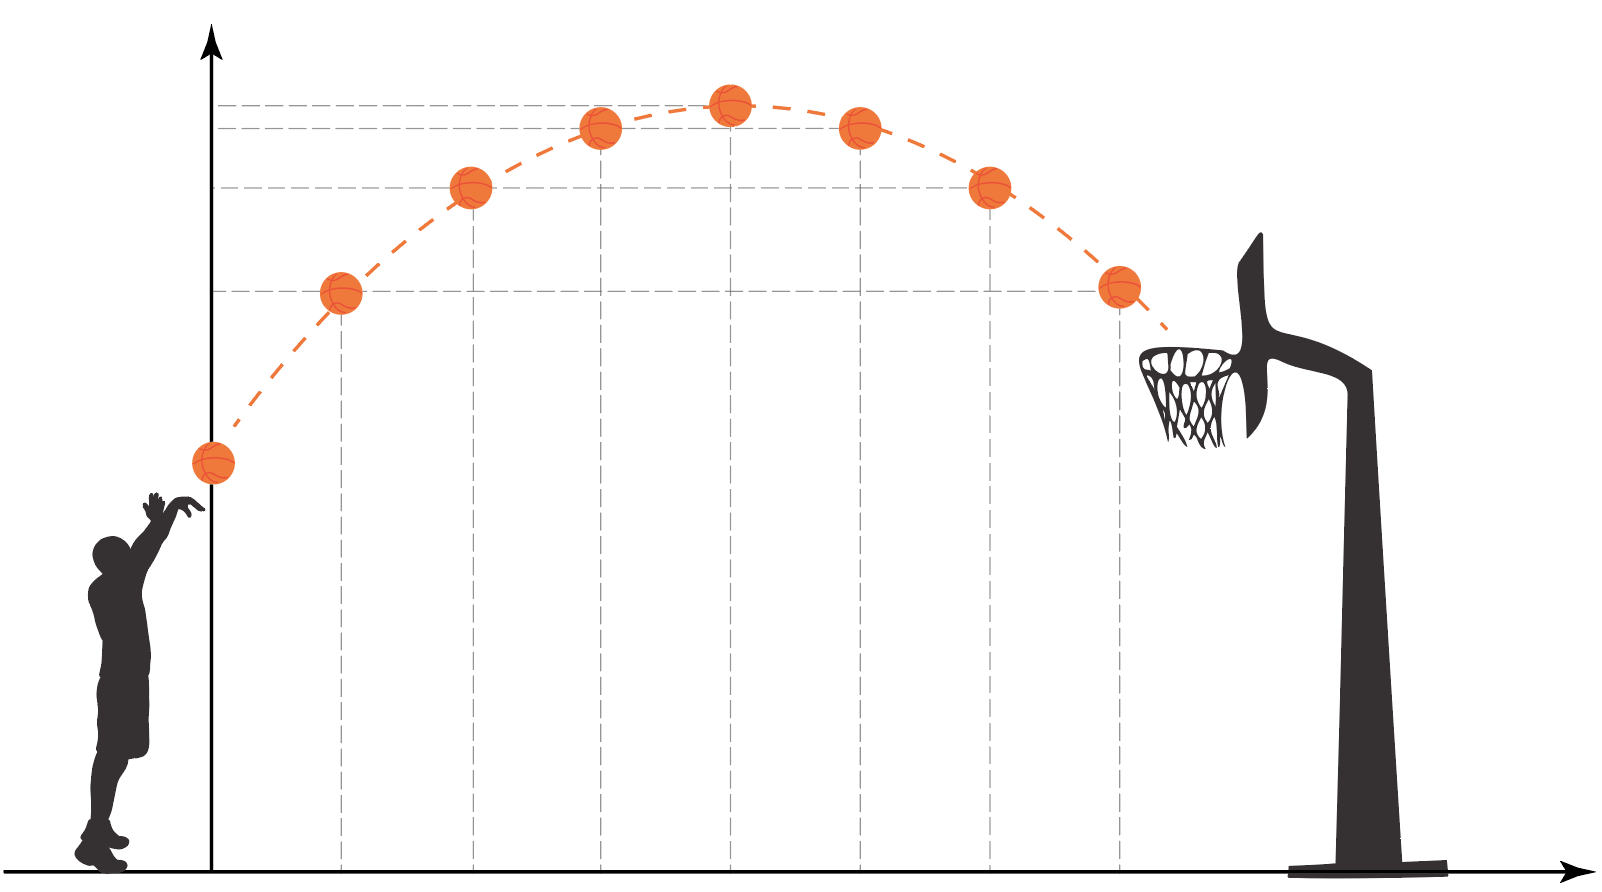
\includegraphics[width=\textwidth]{basquete}  
\end{center}

Admitindo que o jogador lançou a bola de uma altura de $2{,}10m$ com velocidade inicial de $v_0 m/s$ (na direção vertical), a função que fornece a variação da altura da bola em função do tempo é dada pela expressão
\[h(t) = 2,10 + v_0 t - 5t^2\],
cujo gráfico também é uma parábola (representado a seguir apenas para $t\geq 0$):

\begin{figure}[H]
\centering
  \begin{tikzpicture}[xscale=2.8]
    \draw[help lines, thin, gray!30, step=.2] (0,0) grid (2.2,4.2);
    \draw[help lines, thin, gray!70] (0,0) grid (2.2,4.2);
    \draw [->, thick] (0,0) -- (0,4.4);
    \node[left, rotate=90] at (-.25,4) {altura (h)};
    \draw [->, thick] (0,0) -- (2.4,0);
    \node[] at (2,-.7) {tempo (t)};
    \foreach \x in {0.5,1,1.5,2} \draw (\x,.1)  -- (\x,-.1)  node[below] {\x};
    \foreach \y in {1,...,4} \draw (.03571,\y) -- (-.03571,\y) node[left] {\y};        
    \node[below left] at (0,0) {0};
    \draw [ domain=0:1.5, color=session3, smooth, very thick] plot (\x,-5*\x^2 +6*\x + 2.1);
  \end{tikzpicture}

\caption{Gráfico de $h(t)$ para $v_0 = 6m/s$.}
\end{figure}

Com a ajuda de uma calculadora, calcule as taxas de variação médias da altura nos seguintes intervalos de tempo para $v_0 = 6 m/s$ e $v_0 = 7 m/s$:

\begin{table}[H]
  \centering
\begin{tabu} to .7\textwidth{|l|c|c|}
  \hline
  \thead
          & $\bm{v_0 = 6 m/s}$ & $\bm{v_0 = 7 m/s}$ \\
\hline
Entre $t=0$ e $t=1$ & & \\
\hline
Entre $t=0$ e $t=0,1$ & & \\
\hline
Entre $t=0$ e $t=0,01$ & & \\
\hline
Entre $t=0$ e $t=0,001$ & & \\
\hline
Entre $t=0$ e $t=0,0001$ & & \\
\hline
\end{tabu}
\end{table}

\begin{enumerate}
\item Olhando para as sequências de valores obtidos acima, o que se pode conjecturar sobre a tendência que eles apresentam?

  Considerando a velocidade inicial igual a $6m/s$, a bola atinge sua altura máxima de $3{,}9m$ depois de $0{,}6s$ do lançamento. Ou seja, o ponto mais alto do gráfico é o par ordenado $(0{,}6;3{,}9)$. Neste ponto a velocidade na direção vertical é igual a zero (uma vez que aí a bola deixa de subir e passa a descer). Observe, agora, as taxas de variação médias da altura nos seguintes intervalos de tempo:


  \begin{multicols}{2}
    \begin{table}[H]
    \begin{tabu}[l]{|l|c|}
      \hline
      \thead
      & $\bm{v_0 = 6m/s}$ \\
      \hline
      Entre $t=0{,}5$ e $t=0{,}6$  & 0,5 \\
      \hline
      Entre $t=0{,}59$ e $t=0{,}6$  & 0,05 \\
      \hline
      Entre $t=0{,}599$ e $t=0{,}6$  & 0,005 \\
      \hline
      Entre $t=0{,}5999$ e $t=0{,}6$  & 0,0005 \\
      \hline
    \end{tabu}
\end{table}
\begin{table}[H]
    \begin{tabu}[r]{|l|c|}
      \hline
      \thead
      & $\bm{v_0 = 6m/s}$ \\
      \hline
      Entre $t=0{,}6$ e $t=0{,}7$  & -0,5 \\
      \hline
      Entre $t=0{,}6$ e $t=0{,}65$  & -0,25 \\
      \hline
      Entre $t=0{,}6$ e $t=0{,}605$  & -0,025 \\
      \hline
      Entre $t=0{,}6$ e $t=0{,}6005$  & -0,0025 \\
      \hline
    \end{tabu}
  \end{table}
\end{multicols}

  
\item A tendência observada nos valores obtidos acima corrobora a sua conjectura do item anterior? Explique.
\item Calcule a taxa de variação média da função $h(t) = 2{,}1 + 6t -5t^2$ entre os tempos $t=1$ e $t=1 + \alpha$, onde a variável $\alpha$ representa um número real próximo de zero. (A resposta ficará em função de $\alpha$).
\item À medida que o valor de $\alpha$ se aproxima de zero, o que se observa com o valor da taxa de variação média calculada no item anterior? O que esse valor significa no contexto do problema?
\end{enumerate}

\ifdefined\prof

\begin{solucao}


\centering
\begin{tabu} to \textwidth{|l|>{$}c<{$}|>{$}c<{$}|}
\hline
\cellcolor{primario}\textcolor{white}& \cellcolor{primario}\textcolor{white}{\bm{v_0=6m/s}} & \cellcolor{primario}\textcolor{white}{\bm{v_0=7m/s}}\\
\hline
Entre $t=0$ e $=1$ & 1 & 2\\
\hline
Entre $t=0$ e $=0,1$ & 5,5 & 6,5\\
\hline
Entre $t=0$ e $=0,01$ & 5,95 & 6,95\\
\hline
Entre $t=0$ e $=0,001$ & 5,995 & 6,995\\
\hline
Entre $t=0$ e $=0,0001$ & 5,9995 & 6,9995\\
\hline
\end{tabu}
\begin{enumerate}

\item Os valores parecem aproximar-se do valor da velocidade inicial, 6 no primeiro caso e 7 no segundo caso.
\item Sim, pois os valores $t$ estão próximos de $0{,}6$ e as taxas de variação médias dessa vez aproximam-se de zero que é a velocidade no ponto mais alto da trajetória.
\item $\displaystyle\frac{h(1+\alpha)-h(1)}{(1+\alpha)-1}=\frac{2,1+6(1+\alpha)-5(1+\alpha)^2=3{,}1}{\alpha}=\frac{-4\alpha-5\alpha^2}{\alpha}=\frac{\alpha(-4-5\alpha)}{\alpha}=4-5\alpha$

\item À medida que $\alpha$ se aproxima de zero, o valor calculado se aproxima de $-4$, que, de acordo com o observado anteriormente, deve ser a velocidade vertical instantânea no tempo $t=1$. O sinal negativo indica que o movimento é para baixo (sentido contrário ao adotado como positivo).

\centering
\begin{tabu} to \textwidth{|*{7}{>{$}c<{$}|}}
\hline
\cellcolor{primario}\textcolor{white}{\bm{\alpha}} & 0{,}1 & 0{,}01 & 0{,}001 & 10^{-4} & 10^{-5} & 10^{-6} \\
\hline
\cellcolor{primario}\textcolor{white}{\bm{-4-5\alpha}} & -4{,}5 & -4{,}05 & -4{,}005 & -4{,}0005 & -4{,}00005 & -4{,}000005 \\
\hline
\end{tabu}

\begin{tabu} to \textwidth{|*{7}{>{$}c<{$}|}}
\hline
\cellcolor{primario}\textcolor{white}{\bm{\alpha}} & -0{,}1 & -0{,}01 & -0{,}001 & -10^{-4} & -10^{-5} & -10^{-6} \\
\hline
\cellcolor{primario}\textcolor{white}{\bm{-4-5\alpha}} & -3{,}5 & -3{,}95 & -3{,}995 & -3{,}9995 & -3{,}99995 & -3{,}999995 \\
\hline
\end{tabu}

\end{enumerate}


\end{solucao}
\fi

\end{document}